\chapter{Introduction\label{cha:introduction}}
In this chapter, I would like to make an overview of the field and relevant shallow
knowledge so that the readers can have some intuitions about the topic and the motivation
behind. 

\section{Motivation\label{sec:moti}}
% intro to machine learning
\subsection{Context}
In the recent years, \acrfull{ml} has become a powerful tool for computer scientists,
business analysts and other professionals to better improve their works because it can
make use of a large amount of data using probabilistic models. It is able to capture
properties of different objects and events by making observations, which is difficult to
do using human labour or traditional rule-based methods which require manual engineering
works. \acrshort{ml} became popular thanks to the boost of data generation in the
Internet era. 

There are three basic approaches for any \acrshort{ml} problems: Supervised Learning,
Unsupervised Learning and Reinforcement Learning. In any of the approaches, the main job
of the learning machine is to optimize an objective function. In order to achieve that,
the learning machine is given a set of models and pick a model which it considers to be
the best. In a lot of settings, this work is similar to approximating a function on a
population through a sampled set of representatives - the "training set".

% Intro to Deep Learning
There are many different approaches to approximate a function on a dataset. For instance,
the most simple one is to assume that the data is linearly distributed and thus just find
the best linear function $\mathbf{w}x + b$ fitting the data, where $x$ is the data point,
$\mathbf{w}$ the parameter vector and $b$ the bias. There are also more complicated class
of models such as Logistics Regression and Support Vector Machine. The common point for
all of these methods is that we have to find a good vector representation of our data,
otherwise the learning algorithms will not work in the most efficient way. The task is called
``Feature Engineering'', and takes in some cases most of the time of the learning task.

Deep Learning is another method and is currently the one with the most exposure because it
could already beat traditional methods in a lot of different fields from Computer Vision
to Natural Language Processing or Sound Recognition. It is basically a class of functions
which consists of different layers of computing, each of which is supposedly responsible
for learning a specific level of understanding about the objective problem. In most of the
cases, Deep Learning is implemented in different forms of Multi-layer Neural Networks.

% Why learning representations?
\subsection{Representation Learning}
As being mentioned above, a very important step in learning is extracting good features
from the input data. In traditional learning methods, this is crucial because the set of
models only understand the input in vector space. In Deep Learning, this is actually not
that heavy because of techniques such as Convolutional Neural Networks which take directly
the raw data and learn different levels of representations in the hidden layers. However,
having a good representation helps not only simplify the learning task dramatically but
also increase the robustness of the learning engine.

% GAN
\subsection{\acrfull{gan}}
\acrlong{gan}s \cite{gan} are Unsupervised Deep Neural Networks where the learning
engine consists of two competing components: The Generator and the Discriminator. As its
name indicates, the generator tries to generate data from a noise distribution, could be
conditioned on some input or have no conditions; while the discriminator tries to classify
between a real data item and the synthesized one from the generator, under the same
condition. While using supervised losses as components, \acrshort{gan} is usually referred
as an Unsupervised \acrshort{ml} task because it does not try to learn a mapping between
the data and a set of labels. Instead, \acrshort{gan} tries to learn the generalized
distribution of a particular dataset and to be able to draw samples from that
distribution. The distribution that \acrshort{gan}, or particularly the Generator, learns
can be unconditional or conditional. The original idea of \acrshort{gan} is unconditional,
whereas many following-up papers use a conditional version to better train it for specific
tasks. The advantage of \acrshort{gan} comparing to some other altenatives such as
\acrfull{vae} \cite{vae} is that \acrshort{gan} tends to produce more realistic images with less
blurry boundaries, which is a shortcoming of the L2 loss \cite{gan}.
However, because \acrshort{gan} does not minimize a standard loss function between the
outputs and the targets, evaluating it is still a challenge. In many cases, human
evaluation is used.

The nature of probabilistic distribution estimation of \acrshort{gan}s motivates
researchers to utilize it for extracting a representation of a dataset. There are
different ideas on using \acrshort{gan} to improve an \acrshort{ml} task. For instance,
the Generator, who is supposed to capture a probabilistic distribution, can draw new
samples from its knowledge of the data, which potentially enriches the training and
evaluation sets of the \acrshort{ml} task. Furthermore, as the Discriminator is trained to
well classify real data from synthesized data from the Generator, can contain layers with
useful information about the dataset. An simple idea is to take the weight vectors of one
or a few layers before the Softmax as representations for other tasks.

\section{Objective\label{sec:objective}}
The main focus of this Master Thesis is the performance of \acrfull{gan} on RGB-D data,
particularly the Washington RGB-D Dataset \cite{washington_rgbd}. We would like to
find out if \acrshort{gan} is able to generate good object images, particularly useful
images as training items for an Object Recognition engine. In the effort to evaluate if
\acrshort{gan} is able to generating useful data for improving classification performance
or not, the thesis emphasizes on experimenting different ways of training a \acrshort{gan}
to learn from RGB and Depth data and testing the \acrshort{gan} results on another Deep
Network for Object Recognition, which we call the ``Baseline Classifier''.

\section{Scope\label{sec:scope}}
The Thesis focuses on evaluating the performance of a trained \acrshort{gan}'s outputs on
training a standard \acrshort{ml} task. Particularly, the author aims to train
\acrshort{gan}s to learn distributions from the Washington Object RGB-D Dataset
\cite{washington_rgbd}, then evaluate the effect that the \acrshort{gan} data
have in Eitel et al. \cite{eitel}. In all of the experiments, a conditional version
of \acrshort{gan} is used. The original unconditional \acrshort{gan} is not in the scope
of this Thesis.  

\subsection{Using a \acrshort{gan} to learn representations from Washington RGBD Dataset} 
In this thesis, two different settings of \acrshort{gan} are experimented. 

In the first model, the objective of the Generator is to generate a good depth map,
conditioned on an RGB frame of an object. Basically, it is the transformation of an object
from a 2D space to a 3D space. The task of the Discriminator, as usual, is to classify a
real depth image from a depth image produced by the generator.

In the second model, the objective of the Generator is to generate a pair of RGB-D data in
another pose of an item, conditioned on both the RGB and the Depth map. Briefly speaking,
this Generator tries to ``rotate'' the object by an angle. The Discriminator, as usual,
tries to classify the real RGB-D pair from the ``fake'' pair.

\subsection{Training a deep neural network to do object classification}
In this Thesis, we use the work from Eitel et al. \cite{eitel} because of several
reasons. First, it is relevant to our scope; the authors train an Object Recognition
Network using Transfer Learning from CaffeNet, one of the first reference implementation
of AlexNet \cite{alexnet}. Second, its
evaluation is based on same dataset (Washington RGB-D) and in the manner that fits us
(learning from both RGB and Depth data). Finally, it achieves high accuracies (more than
91\% when using both RGB and Depth data).

\subsection{Comparing classification performances on original data and data from
	\acrshort{gan} in different scales}
We perform the evaluation of a \acrshort{gan} in multiple steps. First of all, we
reproduce the paper's \cite{eitel} results by implementing the Classification
Network in Tensorflow.  Second, we substitute a part of training data by the generated
data from the corresponding \acrshort{gan}, in different levels (50\%, 75\%, and 90\%),
and train the Classification Network accordingly. All of the resulting models are tested
on the same fixed Test Set, which we will discuss further in Chapter
\ref{cha:methodology}. Third, we perform some noise injection experiments to the Depth and
RGB components respectively to better understand how much those components contribute to
the classification results.

%'Figure \ref{fig:intro} shows Component X as part of ...' 
%\\
%\begin{figure}[htb]
  %\centering
  %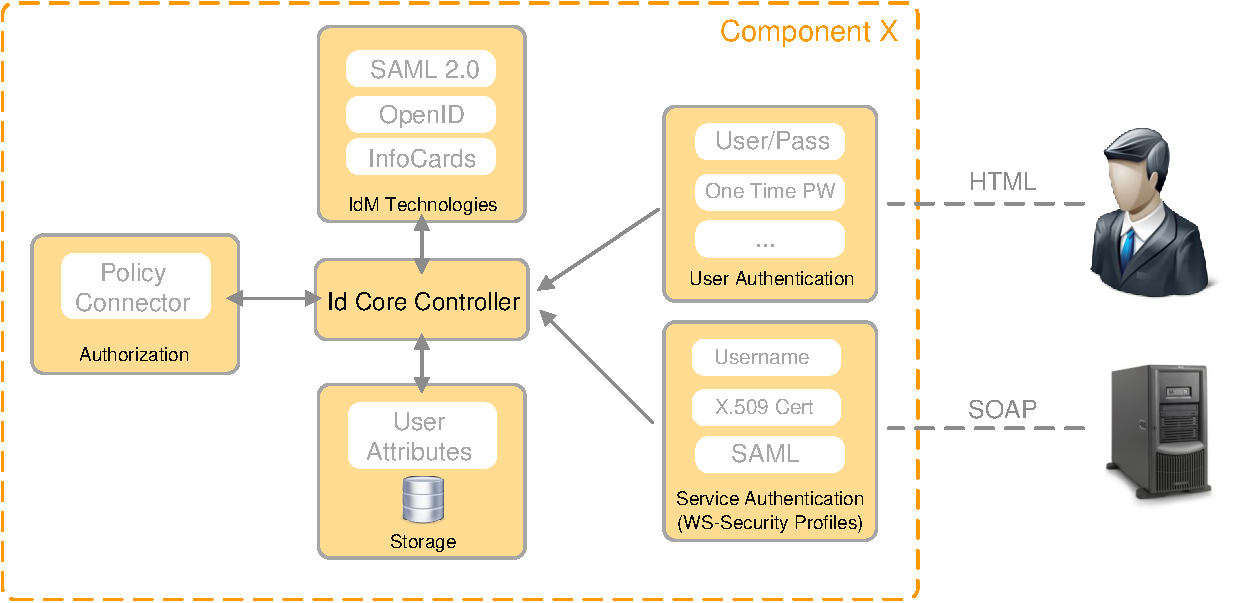
\includegraphics[width=9cm]{intro_example.pdf}\\
  %\caption{Component X}\label{fig:intro}
%\end{figure}

\section{Outline\label{sec:outline}}

This section gives a brief outline of the content of the following chapters in this
thesis.
\\
\\
\textbf{Chapter \ref{cha:relatedwork}} describes the relevant researches and the
foundation works which are used in this thesis. It also gives an introduction to the
background needed to follow the next chapter.
\\
\\
\textbf{Chapter \ref{cha:methodology}} discusses the architectural design of the model
classes we use in this thesis, how we train the models and some relevant theoretical
reasoning. The evaluation strategy and the train-test split are also thoroughly discussed.
\\
\\
\textbf{Chapter \ref{cha:evaluation}} explains how we set up the experiments and
thoroughly analyzes  the evaluation results of our models.
\\
\\
\textbf{Chapter \ref{cha:conclusion}} summarizes the thesis, describes the problems that
occurred and gives an outlook about future work.
